\documentclass[a4paper,10pt]{scrartcl}
\usepackage[utf8]{inputenc}
\usepackage{amsmath,latexsym}
\usepackage[margin=3cm]{geometry}
\usepackage{axodraw2}
\usepackage{listings}
\lstset{basicstyle=\ttfamily,
keywordstyle=\color{magenta},
  showstringspaces=false
}

\renewcommand{\baselinestretch}{1.5}

\title{Documentation of GPT for QPDFs \newline Part II: Specifics for Measuring DA/FF/QPDF}
\author{Philipp Scior}
\date{\today}
\newcommand{\tr}{\text{Tr\,}}
\newcommand{\bs}{\boldsymbol}
\definecolor{mygreen}{rgb}{0,0.6,0}
\definecolor{mygray}{rgb}{0.5,0.5,0.5}

\begin{document}
\maketitle

This is part II of the documentation, where I explain both our general approach to measuring a pion DA and go over the GPT code for measuring it
using Domain-Wall fermions with a deflated inverter on one of the 96I ensembles by RBC.

\section{GPT\_QPDF\_Utils}
All the necessary functionalities to measure correlators for pion DA or FF/QPDF are contained in the 
gpt\_qpdf\_utils.py module. This module will again need gpt and numpy as imports. There is a globaly defined,
ordered list containing tags for labeling the gamma-matrix channels in the correlator output. \newline
The basic functionalities for the measurement of pion related correlators are defined in the pion\_measurement
base class. All other pion measurement classes will be derived from the pion\_measurement class and inherit it's
members.
\subsection{class pion\_measurement}
\begin{itemize}
    \item Data members: These are basically all parameters for the measurements:
        \begin{itemize}
            \item plist = list of lattice momenta to be used in contractions ([int, int, int, int]).
            \item width = width of gaussian smeared source (double).
            \item pos\_boost = boost for smeared sources used for forward propagators ([int, int, int]).
            \item neg\_boost = boost for smeared sources used for backward propagators ([int, int, int]).
            \item save\_propagators = boolean flag for saving propagators to disk.
        \end{itemize}
    \item \lstinline{__init__(self, parameters)}: Constructor for the class, sets the parameters.
    \item \lstinline{set_output_facilites(self, corr_file, prop_file)}: open the files for propagator- and
            correlator-IO.
    \item \lstinline{propagator_output(self, tag, prop_f, prop_b)}: does the IO for a pair of forward and
            backward propagator. "tag" should be a unique identifier string for the propagator pair.
    \item \lstinline{make_96I_inverter(self, U, evec_file)}: generates inverters for RBC's 96I lattices.
           Needs the gauge field and the path to the file contatining Eigenvectors as input. \newline \textbf{returns:}
           exact inverter, sloppy inverter, object for pinning EVs to GPU memory. 
    \item  \lstinline{make_debugging_inverter(self, U)}: generates simplified inverters for debugging.
    \item \lstinline{make_mom_phases(self, grid, L)}: generates a list of complex fields containing phases for
            projecting onto non-zero momentum. Needs the grid as input. \newline \textbf{returns:} list of complex phase fields, length pzmax-pzmin.
    \item \lstinline{create_WL(self, U)}: \textbf{returns:} a list of Wilson loops in z-direction from length 0 to zmax. 
    \item \lstinline{contract_2pt(self, prop_f, prop_b, phases, trafo, tag)}: applies sink smearing to propagators, 
    does contraction for "pion" 2pt functions (contractions for all momenta in plist and all 16 gamma matrices). Finally also does
    the correlator output to disk.
    \newline \textbf{input:} forw. prop., backw. prop., list of phases, gf. matrices, unique tag)
    \item \lstinline{create_src_2pt(self, pos, trafo, grid)}: makes 2 gaussian smeared, boosted source for forward and backward prop.
            \newline \textbf{input:} position of source, gf. matrices, grid.
            \newline \textbf{returns:} two fermion propagator containing the sources.
\end{itemize}


\section{Pion Distribution Amplitude}
Let us start by defining the equal-time matrix element needed to determine the pion quasi-DA:
\begin{equation}
    \langle 0 | \bar d(z) \gamma_z \gamma_5 W(z,x) u(x) | \pi^+ (p) \rangle 
\end{equation}
Or in other terms
\begin{align}
     =& \langle 0 | \bar d(z) \gamma_z \gamma_5 W(z,x) u(x) \sum_{\vec y} e^{-i \vec p \vec y} \bar u^{S,+k}(y) \gamma_5 d^{S,-k}(y)| 0 \rangle \; , \\
     =& \sum_{\vec y} e^{-i \vec p \vec y} \; \tr \left[ \gamma_5 D^{SP,-k}(y,z) W(z,x) \gamma_z \gamma_5 D^{PS,+k}(x,y) \right] \; .
    % \sum_{\vec y} e^{-i \vec p \vec y} \; \tr\left[ G^{SP, + \vec k}(y;\vec x, t) W(x,z) \gamma_z \gamma_5  G^{PS, -\vec k}(\vec z, t ; y)   \gamma_5 \right] \; ,
\end{align}
where z is short hand notation for $x+ z \vec e_z$, G(x,y) is a propagator from y to x, W(y,x) is a Wilson line from x to y. S and P denote a smeared or point src or sink, where k is the boost momentum 
used in the respective smearing kernel. Now, we rewrite the expression by interchanging the summation variable using translational invariance, using $\gamma_5$ hermiticity and
$W(x,y) = W^\dagger(y,x)$
\begin{align}
    =& \sum_{\vec x} e^{-i \vec p \vec x} \; \tr \left[ \gamma_5 D^{SP,-k}(y,z) W(z,x) \gamma_z \gamma_5 D^{PS,+k}(x,y) \right] \; , \\
    =& \sum_{\vec x} e^{-i \vec p \vec x} \; \tr \left[ D^{PS,-k}(z,y)^\dagger W(x,z)^\dagger \gamma_z D^{PS,+k}(x,y) \right] \; , \\
    =& \sum_{\vec x} e^{-i \vec p \vec x} \; \tr \left[ (W(x,z) D^{PS,-k}(z,y))^\dagger \gamma_z D^{PS,+k}(x,y) \right] \; .
\end{align}
We also have to normalize this DA two-point function by the pion two-point function, i.e. we have to compute:
\begin{align}
    \langle \pi (p) | \pi(p) \rangle & = \sum_{\vec x} e^{-i \vec p (\vec x - \vec y)} \; \tr \left[ D^{SS , +\vec k}(x,y) \left( D^{SS, -\vec k}(x,y)\right)^\dagger \right] \; .
\end{align}
In this case we use smeared-smeared Propagators for determining the pion two-pint function but maybe we only need point-smeared. 
We can reuse both propagators from the DA two-point function for the pion two-point function, saving the cost of two inversion, and apply additional smearing
to the sink.
\subsection{Computational Strategy}
The strategy to compute the pion DA is the following:
\begin{itemize}
    \item Generate two smeared, boosted sources ($+k$, $-k$) at $y$.
    \item Make two propagators $y \to all$.
    \item Make an array containing fields of Wilson loops from $all \to all +z \vec e_z$, $\forall z$.
    \item $\forall z$:
    \begin{itemize}
        \item Shift backwards propagator from pion 2pt function covariantly by $+z \vec e_z$.
        \item Construct DA backwards propagator by : $(W(x,z) * \text{shifted prop. from step before} )^\dagger$
        \item Multiply propagators, Dirac matrix, phase. Take trace, reduce
    \end{itemize}
\end{itemize}
In the following I will go over the DA.py file used to measure both two-point functions needed for DA. I will not describe parts of the program handling input parameters
like e.g. filenames or how to handle or bundle running of multiple jobs. Instead I will focus on the used functions.
\subsection{class pion\_DA\_measurement}
A class derived from the pion\_measurement base class. Contains the additional functions:
\begin{itemize}
    \item Data members: These are basically all parameters for the measurements:
        \begin{itemize}
            \item zmax = Max. length of the Wilson loop in z-direction (int).
            \item pzmin = minimal lattice momentum in z-direction (int).
            \item pzmax = maximal lattice momentum in z-direction (int).
            \item plist = list of lattice momenta in z-direction between pzmin and pzmax.
            \item width = width of gaussian smeared source (double).
            \item pos\_boost = boost for smeared sources used for forward propagators ([int, int, int]).
            \item neg\_boost = boost for smeared sources used for backward propagators ([int, int, int]).
            \item save\_propagators = boolean flag for saving propagators to disk.
        \end{itemize}
    \item \lstinline{constr_backw_prop_for_DA(self, prop_b, W)}: constructs a list of "backwards propagators"
            to be used as backwards propagators in contract\_DA. \newline \textbf{returns:}  {[} (W[z] *prop\_b )$^\dagger$ for all z in range(0,zmax){]}
    \item \lstinline{contract_DA(self, prop_f, prop_b, phases, tag)}: does the contractions for the DA 2pt function and handles correlator output.
            \newline \textbf{input:} forw. prop, list of backw. props, list of momentum phases, unique identifier string) 
\end{itemize}

\subsection{Driver Code}

\lstinputlisting[language=Python,basicstyle=\footnotesize,commentstyle=\color{mygreen},numbers=left,numberstyle=\tiny\color{mygray},]{DA.py}


\section{Pion Form Factor/ quasi-PDF}
Let us start by defining the matrix element (3pt function) needed for both determinations:
\begin{equation}
    C_{3pt}(\vec p_f,\vec p_i,\tau,t_f-t_i,L) = \langle \Pi (\vec p_f, t_f) O_{\Gamma}(\tau) \Pi^\dagger (\vec p_i, t_i) \rangle \; , \label{3pt}
\end{equation}
with the insertion operator:
\begin{equation}
    O_\Gamma(\tau) = \sum_{\vec z} e^{i \vec q \vec z} \left[ \bar u_z W_{z,z+L} \Gamma u_{z+L} - \bar d_z W_{z,z+L} \Gamma d_{z+L} \right] \; , \label{insert}
\end{equation}
where $q$ is the momentum transfer. Now, we need to distinguish between whats needed for the FF and the QPDF:
\begin{align}
    \text{FF}: \quad & C_{3pt}(\vec p_f,\vec p_i,\tau,t_f-t_i,L=0) \quad \text{with } O_{\gamma_t} \; , \\
    \text{QPDF:} \quad & C_{3pt}(\vec p,\vec p,\tau,t_f-t_i,L) \; .
\end{align}
For the FF we have $\vec p_f = \vec p_i + \vec q$ and in the insertion operator we have a local operator
without a Wilson line connecting the quark operators ($L=0$) and we are only interested in the $\gamma_t$ channel. Where for the QPDF
we have no momentum transfer between in and out states, i.e. $\vec p_f = \vec p_i = \vec p$ and a Wilson line of length $L$. We will now write down the most general
from of the 3pt function in eq.\eqref{3pt} that can be used for measurements of both FF and QPDF by adjusting the necessary parameters.
\begin{align}
    C_{3pt}(\vec p_f,&\vec p_i,\tau,t_f-t_i,L) = \langle \Pi (\vec p_f, t_f) O_{\Gamma}(\tau) \Pi^\dagger (\vec p_i, t_i) \rangle \; , \\
    &= \sum_{\vec y, \vec z} e^{-i \vec p_f y} e^{i \vec p_i \vec x} e^{i \vec q \vec z} \langle \left[\bar d^{-l}_y \gamma_5 u^l_y \right] \bar u_z W_{z,z+L} \Gamma u_{z+L}
    \left[\bar u^k_x \gamma_5 d^{-k}_y \right] \rangle \; ,\\
    &= \sum_{\vec y, \vec z} e^{-i \vec p_f \vec y} e^{i \vec p_i \vec x} e^{i \vec q \vec z} \tr \left[ W_{z,z+L} \Gamma D^u_{z+L,x''} S^k_{x'',x} \gamma_5
            S^{-k}_{x,x'} D^d_{x',y'} S^{-l}_{y',y} \gamma_5 S^l_{y,y''} D^u_{y'',z}   \right] \; , \\
    &= \sum_{\vec{z}} e^{i \vec q \vec z} \tr \left[B^{y_4,\vec p_f, \vec p_i}_{x,z} W_{z,z+L} \Gamma F_{z+L,x} \right] \; ,
\end{align}
with the forward and (sequential-) backward propagators:
\begin{align}
    F_{z+L,x} &= D^u_{z+L,x''} S^k_{x'',x} \;, \\
    B^{y_4,\vec p_f, \vec p_i}_{x,z} &= \sum_{\vec y} e^{-i \vec p_f \vec y} e^{i \vec p_i \vec x} \gamma_5 S^{-k}_{x,x'} D^d_{x',y'} S^{-l}_{y',y} \gamma_5 S^l_{y,y''} D^u_{y'',z} \;.
\end{align} 
Where the $S^k$ stand for gaussian smearing operators with boost momentum $k$. This is of course only the contribution for the up quark in the
insertion operator and in principle there is also a disconnected contribution to the 3pt function. However, in the full expression for u-d with 
degenerate u and d quarks the disconnected contributions cancel while the connected contribution for d is either the hermitian conjugate of the u contribution or 
-1 * hermitian conjugate, depending on the gamma matrix in the insertion operator.
\newline
For the QPDF matrix element we have $\vec p_f = \vec p_i = \vec p$ and therefore momentum transfer $\vec q = 0$ and also equal boost momenta in
the external pion states:
\begin{align}
    C_{3pt}(\vec p,y_4,t_f-t_i,L) &=  \sum_{\vec{z}} \tr \left[B^{y_4,\vec p}_{x,z} W_{z,z+L} \Gamma F_{z+L,x} \right] \;  \\
    F_{z+L,x} &= D^u_{z+L,x''} S^k_{x'',x} \;, \\
    B^{y_4,\vec p}_{x,z} &= \sum_{\vec y} e^{-i \vec p ( \vec y- \vec x)} \gamma_5 S^{-k}_{x,x'} D^d_{x',y'} S^{-k}_{y',y} \gamma_5 S^k_{y,y''} D^u_{y'',z} \;.
\end{align}
For the FF matrix element we have $\vec p_f = \vec p_i + \vec q$ and we find:
\begin{align}
    C_{3pt}(\vec p_f, \vec{p}_i,y_4,t_f-t_i) &=  \sum_{\vec{z}} e^{- i \vec q \vec z} \tr \left[B^{y_4,\vec p}_{x,z} \gamma_t F_{z+L,x} \right] \;  \\
    F_{z,x} &= D^u_{z,x''} S^k_{x'',x} \;, \\
    B^{y_4,\vec p}_{x,z} &= \sum_{\vec y} e^{-i \vec p_f\vec y} e^{i \vec p_i\vec x} \gamma_5 S^{-k}_{x,x'} D^d_{x',y'} S^{-l}_{y',y} \gamma_5 S^{l}_{y,y''} D^u_{y'',z} \;.
\end{align}

\subsection{Computational Strategy}
In the following we will go over the strategy to compute the pion FF/ QPDF \& the 2pt-function. In order to do this, let us first derive how to calculate the (sequential) backward propagator:
\begin{align}
    B^{y_4,\vec p_f, \vec p_i}_{x,z} &= \sum_{\vec y} e^{-i \vec p_f \vec y} e^{i \vec p_i \vec x} \gamma_5 \underbrace{
    S^{-k}_{x,x'} D^d_{x',y'} S^{-l}_{y',y} 
    \gamma_5 S^l_{y,y''} D^u_{y'',z}}_{Q_y(x,z)}  \;, \\
    \gamma_5 Q_y(x,z) \gamma_5 &= \gamma_5 S^{-k}_{x,x'} D^d_{x',y'} \gamma_5 S^{-l}_{y',y} \gamma_5 S^l_{y,y''} \gamma_5 D^u_{y'',z} \gamma_5 \; ,\\
    &= D^{u \dagger}_{z,y''} S^l_{y'',y} \gamma_5 S^{-l}_{y,y'}D^{d \dagger}_{y',x'} S^{-k}_{x',x} \; , \\
    &= Q^\dagger_y(z,x) \; , \\
    \Rightarrow B^{y_4,\vec p_f, \vec p_i}_{x,z} &= \sum_{\vec y} e^{-i \vec p_f \vec y} e^{i \vec p_i \vec x} Q_y^\dagger(z,x) \gamma_5 \; ,
\end{align}
where we used $\gamma_5$ hermiticity and the fact that the smearing kernel is hermitian. Now the overall strategy is:
\begin{itemize}
    \item Generate two smeared, boosted sources ($+k$, $-k$) at $x$.
    \item Make two propagators $x \to all$.
    \item Smear both propagators at sink and make 2pt function.
    \item Compute backwards sequential propagator:
    \begin{itemize}
        \item Reuse point-smeared backw. prop. from pion 2pt function.
        \item Smear sink
        \item Set sequential source at $t_{op}$ $=$ propagator at $t_{op}$
        \item Smear sequential source
        \item $\gamma_5 \; \times$ smeared sequential source
        \item Multiply the right phases (complex conjugate!)
        \item Performing inversion on this sequential source
    \end{itemize}
    \item Use $B^\dagger$ in contraction 
    \item Reuse forward propagator from 2pt function (only PS not SS)
    \item[*] Make an array containing fields of Wilson loops from $all \to all +z \vec e_z$, $\forall z$.
    \item[*] $\forall z$:
    \begin{itemize}
        \item Shift Forward propagator covariantly by $+z \vec e_z$.
        \item Multiply forward propagators and Wilson loop($z$)s.
    \end{itemize}
    \item Contract everything.
\end{itemize}
The steps marked with (*) are only for the QPDF calculation and have to be omitted for the FF. Overall we need two inversions for the 2pt function
and one additional inversion for the backwards propagator in the 3pt function. Looking at all the steps we recognize that 
most steps are similar to those from the DA calculation, only the construction of the backward propagator and the final contraction differ
from their counterparts in the DA calculation. Therefore the gpt\_qpdf\_utils module contains two other classes derived from the base measurement class,
which will be defined below. 

\subsection{class pion\_ff\_measurement}
\begin{itemize}
    \item Data members:
        \begin{itemize}
            \item p = momentum of the outgoing pion (z-direction) in lattice units ([int, int, int, int]).
            \item q = momentum transfer (z-direction) in lattice units ([int, int, int, int]).
            \item plist = a list of the q's. This is just for internal handeling of the momenta in the contraction algorithm. Do not change.
            \item t\_insert = insertion time of the operator (int).
            \item width = width of gaussian smeared source (double).
            \item boost\_in = boost for the quarks in in-going pion ([int, int, int]).   
            \item boost\_out = boost fror the quarks in the out-going pion ([int, int, int]).
            \item pos\_boost = boost for smeared sources used for forward propagators derived from boost\_in.
            \item neg\_boost = boost for smeared sources used for backward propagators derived from boost\_in.
            \item save\_propagators = boolean flag for saving propagators to disk.
        \end{itemize}
    \item \lstinline{contract_FF(self, prop_f, prop_b, phases, tag)}: Does the contraction of the FF 3pt function and handles the correlator output.
    \item \lstinline{create_bw_seq(self, inverter, pos, grid, trafo)}: Computes the sequential backward propagator start at pos through t\_insert. 
            \newline \textbf{input:} inverter, source position, grid, gauge trafo. field.
            \newline \textbf{returns:} sequential backward propagator.
\end{itemize}

\subsection{Driver Code}

\lstinputlisting[language=Python,basicstyle=\footnotesize,commentstyle=\color{mygreen},numbers=left,numberstyle=\tiny\color{mygray},]{FF.py}

\subsection{class pion\_qpdf\_measurement}
\begin{itemize}
    \item Data members:
        \begin{itemize}
            \item zmax = max. length of the Wilson line (int).
            \item p = momentum of the outgoing pion (z-direction) in lattice units ([int, int, int, int]).
            \item q = momentum transfer (z-direction) in lattice units ([int, int, int, int]).
            \item plist = a list of the q's. This is just for internal handeling of the momenta in the contraction algorithm. Do not change.
            \item t\_insert = insertion time of the operator (int).
            \item width = width of gaussian smeared source (double).
            \item boost\_in = boost for the quarks in in-going pion ([int, int, int]).   
            \item boost\_out = boost fror the quarks in the out-going pion ([int, int, int]).
            \item pos\_boost = boost for smeared sources used for forward propagators derived from boost\_in.
            \item neg\_boost = boost for smeared sources used for backward propagators derived from boost\_in.
            \item save\_propagators = boolean flag for saving propagators to disk.
        \end{itemize}
    \item \lstinline{contract_QPDF(self, prop_f, prop_b, phases, tag)}: Does the contraction of the QPDF 3pt function and handles the correlator output.
    \item \lstinline{create_fw_prop_QPDF(self, prop_f, W)}: Does the multiplication of Wilson line and the shifted forward propagator.
           \newline \textbf{return:} List of W * forward propagator.
    \item \lstinline{create_bw_seq(self, inverter, pos, grid, trafo)}: Computes the sequential backward propagator start at pos through t\_insert. 
            \newline \textbf{input:} inverter, source position, grid, gauge trafo. field.
            \newline \textbf{returns:} sequential backward propagator.
\end{itemize}

\subsection{Driver Code}

\lstinputlisting[language=Python,basicstyle=\footnotesize,commentstyle=\color{mygreen},numbers=left,numberstyle=\tiny\color{mygray},]{QPDF.py}

\section{Proton quasi-PDF}
The Matrix-element for the proton qPDF is
\begin{align}
    M = \langle \text{proton}(p_f) | O_\Gamma(z,\tau) | \text{proton}(p_i) \rangle \; ,
\end{align}
with the proton in- and out-states:
\begin{align}
    | \text{proton}(x) \rangle &= \epsilon_{abc} (\bar u^\alpha_a(x) [C \gamma_5]^{\alpha \beta} \bar d^{\beta T}_b(x)) \bar u^\gamma_c(x) P^{\gamma \delta} \; , \\
    \langle \text{proton}(y) | &= \epsilon_{a'b'c'} P^{\delta \gamma'} u^{\gamma'}_{c'}(y) (u^{\alpha' T}_{a'}(y) [C \gamma_5]^{\alpha' \beta'} d^{\beta'}_{b'}(y) ) \; ,
\end{align}
where $C=i \gamma_2 \gamma_4$ is the charge conjugation operator and $P$ is a projector onto a fixed parity \& polarization state. We will use the three different projectors   
\begin{align}
    P_{+,S_z+} &= \frac{1}{4} (1+ \gamma_4)(1-i\gamma_1 \gamma_2) \;, \notag \\
    P_{+,S_x+} &= \frac{1}{4} (1+ \gamma_4)(1-i\gamma_2 \gamma_3) \; ,\\
    P_{+,S_x-} &= \frac{1}{4} (1+ \gamma_4)(1+i\gamma_2 \gamma_3) \;, \notag
\end{align}
while we are using a more "textbookish" version for the Diract matrix convention, the correlation functions with these definitions are (up to a sign and a factor of 4) compatible with those 
in the QLUA code. The insertion operator is the same as in eq.~\eqref{insert}. Using smearing for the quarks in the external 
states we find the 3pt function associated with this matrix element to be:
\begin{align}
    C_{3pt}(\vec p_f, \vec p_i, \vec q, \tau, t, z) =& \sum_{\vec y, \vec w} e^{-i \vec p_f \vec y} e^{i \vec p_i \vec x} e^{i \vec q \vec w} \epsilon_{abc} \epsilon_{a'b'c'} \notag
    P^{\gamma' \gamma} [C \gamma_5]^{\alpha' \beta'} [C \gamma_5]^{\alpha \beta} \Gamma^{\mu \epsilon} W_{de}(x, x+L) \notag \\
    & \left( -(S_{y,y'}^l D_{y',x'}S^k_{x',x})^{\beta' \beta}_{b'b} \right. \notag \\
    &\Big\lbrace (S_{y,y'}^l D_{y',w})^{\alpha' \mu}_{a'd} \Big[ (D_{w+l,x'}S^k_{x',x})^{\epsilon \alpha}_{ea} (S_{y,y'}^l D_{y',x'}S^k_{x',x})^{\gamma' \gamma}_{c'c} \notag \\
    & \qquad \qquad \qquad \; - (D_{w+l,x'}S^k_{x',x})^{\epsilon \gamma}_{ec} (S_{y,y'}^l D_{y',x'}S^k_{x',x})^{\gamma' \alpha}_{c'a} \Big] \label{3pt_general} \\
    & -(S_{y,y'}^l D_{y',w})^{\gamma' \mu}_{c'd} \Big[ (D_{w+l,x'}S^k_{x',x})^{\epsilon \alpha}_{ea} (S_{y,y'}^l D_{y',x'}S^k_{x',x})^{\alpha' \gamma}_{a'c} \notag \\
    & \qquad \qquad \qquad \; - (D_{w+l,x'}S^k_{x',x})^{\epsilon \gamma}_{ec} (S_{y,y'}^l D_{y',x'}S^k_{x',x})^{\alpha' \alpha}_{a'a} \Big] \Big \rbrace\notag \\
    & + (S^l_{y,y'} D_{y',w})^{\beta'\mu}_{b'd} (D_{w+L,x'}S^k_{x',x})^{\epsilon \beta}_{e,b} \Big[ (S^l_{y,y'}D_{y',x'}S^k_{x',x})^{\gamma' \gamma}_{c'c}
    (S^l_{y,y'}D_{y',x'}S^k_{x',x})^{\alpha' \alpha}_{a'a} \notag \\
    & \qquad \qquad - \left. (S^l_{y,y'}D_{y',x'}S^k_{x',x})^{\gamma' \alpha}_{c'a} (S^l_{y,y'}D_{y',x'}S^k_{x',x})^{\alpha' \gamma}_{a'c} \Big] \right) \notag \; .
\end{align}
The disconnected contribution from the up- \& down-pieces cancel, however the connected pieces combine in a non-trivial way (there is also a cancelation
between one of the up- and one of the down-terms but obviously they do not cancel completely). 
We probably also need the 2pt function for normalization. It is given by:
\begin{align}
C_{2pt}(\vec p,t) &= \sum_{\vec y} e^{-i \vec p (\vec y - \vec x)} \epsilon_{abc} \epsilon_{a'b'c'} P^{\gamma' \gamma} [C \gamma_5]^{\alpha' \beta'} [C \gamma_5]^{\alpha \beta}
                    (S_{y,y'}^k D_{y',x'}S^k_{x',x})^{\beta' \beta}_{b'b} \notag \\
                & \qquad \qquad \qquad \Big \lbrace (S_{y,y'}^k D_{y',x'}S^k_{x',x})^{\alpha' \alpha}_{a'a} (S_{y,y'}^l D_{y',x'}S^k_{x',x})^{\gamma' \gamma}_{c'c} \\
                & \qquad \qquad \qquad -(S_{y,y'}^l D_{y',x'}S^k_{x',x})^{\gamma' \alpha}_{c'a} (S_{y,y'}^l D_{y',x'}S^k_{x',x})^{\alpha' \gamma}_{a'c} \Big \rbrace \notag \; .
\end{align}
by introducing
\begin{equation}
    F = S^l_{y,y'} D_{y',x'} S^k_{x',x} \;,
\end{equation}
we can write the 2pt function as 
\begin{align}
    C_{2pt}(\vec p,t) = \sum_{\vec y} e^{-i \vec p (\vec y - \vec x)} &\epsilon_{abc} \epsilon_{a'b'c'} \notag \\
    (C\gamma_5 F C\gamma_5)^{\alpha' \alpha}_{b'b} \Big \lbrace & F^{\alpha' \alpha}_{a'a} (PF)^{\gamma \gamma}_{c'c} - (PF)^{\gamma \alpha}_{c'a} F^{\alpha' \gamma}_{a'c} \Big \rbrace \;.
\end{align}
I am not quite sure about the global sign of 2pt and 3pt function but the "sign convention" is consistent.
\subsection{Strategy for Contractions}
\begin{figure}[ht]
    \begin{minipage}[b]{0.45\linewidth}
    \centering
    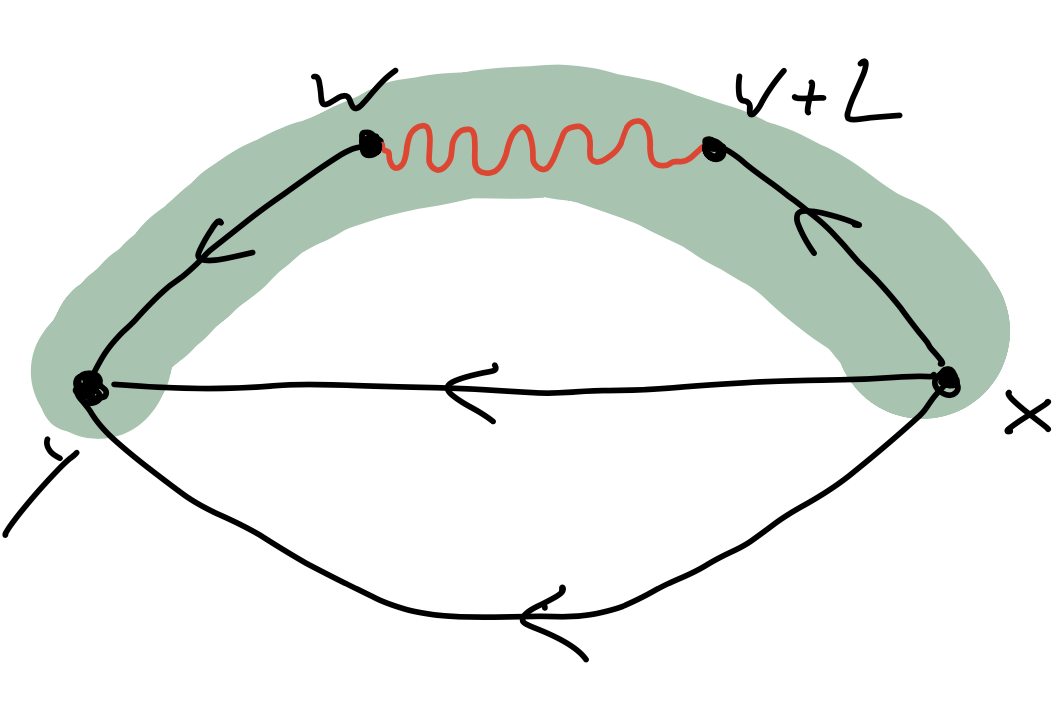
\includegraphics[width=\textwidth]{stratA.png}
    \end{minipage}
    \hspace{0.5cm}
    \begin{minipage}[b]{0.45\linewidth}
    \centering
    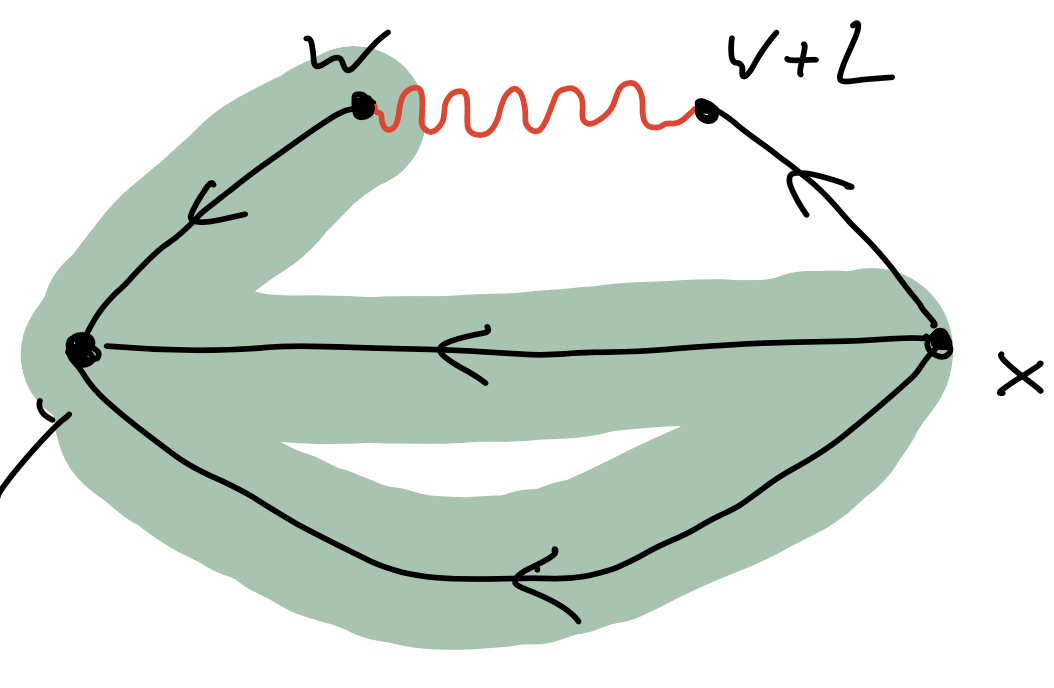
\includegraphics[width=\textwidth]{stratB.png}
    \end{minipage}
    \caption{Left: Contraction strategy A. Right: Contraction strategy B. The greenly shaded parts of the diagram indicate the sequential propagator.}
\end{figure}
Contracting the 2pt function is straight forward. However, there are two possible strategies for contracting the 3pt functions. It basically boils down
to how to do the sequential propagators. Either choice comes with it's up- and down-sides.
\subsection{Strategy A}
Here we do the sequential solve trough the operator insertion. We now introduce the sequential propagator
we introduce:
\begin{align}
    Q &= \sum_{\vec w} e^{i \vec q \vec w} S^l_{y,y'} D_{y',w} \Gamma W(w, w+L) D_{w+L,x'} S^k_{x',x} \; ,   
\end{align}
with this the 3pt function reads:
\begin{align}
    C_{3pt}(\vec p_f, \vec p_i, \vec q, \tau, t, z) = \sum_{\vec y, \vec w} e^{-i \vec p_f \vec y} &e^{i \vec p_i \vec x} \epsilon_{abc} \epsilon_{a'b'c'} \Biggl(\notag \\
    -(C\gamma_5 F C\gamma_5)^{\alpha' \alpha}_{b'b} \Big \lbrace &Q^{\alpha' \alpha}_{a'a} (PF)^{\gamma \gamma}_{c'c} - Q^{\alpha' \gamma}_{a'c} (P F)^{\gamma \alpha}_{c'a} \notag\\
    + &F^{\alpha' \alpha}_{a'a} (PQ)^{\gamma \gamma}_{c'c} - F^{\alpha' \gamma}_{a'c} (P Q)^{\gamma \alpha}_{c'a} \Big \rbrace  \\
    + (C\gamma_5 Q C\gamma_5)^{\alpha' \alpha}_{b'b} \Big \lbrace & (PF)^{\gamma \gamma}_{c'c} F^{\alpha' \alpha}_{a'a} - F^{\alpha' \gamma}_{a'c} (PF)^{\gamma \alpha}_{c'a} \Big \rbrace \Biggr) \notag \; .
\end{align}
This is pretty easy to implement and we can do the contractions for all source-sink separations at the same time. However, we need an inversion for each
combination of gamma matrix and Wilson loop length. Overall we need $((z_\text{max}) \; \times \; \#\text{Gammas} \; + \;1)$ inversions for the determination of the proton qPDF, 
one for the regular forward propagator and all other additional inversions for the sequential forward propagator
in the 3pt function, where $z_\text{max}$ is the maximal length of the Wilson loop. \newline
\subsection{Strategy B}
Here we do the sequential solve through the sink. The derivation is similar to the one in arXiv:hep-lat/0201021.pdf. To be able to do this in a compact and readable way, we will fist restate eq.~\eqref{3pt_general} in a more compact form
by dropping the indices associated to smearing:
\begin{align}
    C_{3pt}(\vec p_f, \vec p_i, \vec q, \tau, t, z) =& \sum_{\vec y, \vec w} e^{-i \vec p_f \vec y} e^{i \vec p_i \vec x} e^{i \vec q \vec w} \epsilon_{abc} \epsilon_{a'b'c'} \notag
    P^{\gamma' \gamma} [C \gamma_5]^{\alpha' \beta'} [C \gamma_5]^{\alpha \beta} \Gamma^{\mu \epsilon} W_{de}(x, x+L) \notag \\
    & \left( -(F_{y,x})^{\beta' \beta}_{b'b} \right. \notag \\
    &\Big\lbrace (D^{SP}_{y,w})^{\alpha' \mu}_{a'd} \Big[ (D^{PS}_{w+l,x})^{\epsilon \alpha}_{ea} (F_{y,x})^{\gamma' \gamma}_{c'c}
     - (D^{PS}_{w+l,x})^{\epsilon \gamma}_{ec} (F_{y,x})^{\gamma' \alpha}_{c'a} \Big] \label{3pt_short}\\
    & -(D^{SP}_{y,w})^{\gamma' \mu}_{c'd} \Big[ (D^{PS}_{w+l,x})^{\epsilon \alpha}_{ea} (F_{y,x})^{\alpha' \gamma}_{a'c}
     - (D^{PS}_{w+l,x})^{\epsilon \gamma}_{ec} (F_{y,x})^{\alpha' \alpha}_{a'a} \Big] \Big \rbrace\notag \\
    & + (D^{SP}_{y,w})^{\beta'\mu}_{b'd} (D^{PS}_{w+L,x})^{\epsilon \beta}_{e,b} \Big[ (F_{y,x})^{\gamma' \gamma}_{c'c}
    (F_{y,x})^{\alpha' \alpha}_{a'a}
     - \left. (F_{y,x})^{\gamma' \alpha}_{c'a} (F_{y,x})^{\alpha' \gamma}_{a'c} \Big] \right) \notag \; .
\end{align}
Now we can reorder a lot of indices and introduce
\begin{align}
    (O_{w,w+L})^{\mu \epsilon}_{de} &= \Gamma^{\mu \epsilon} W(w,w+L)_{de} \; , \\ 
    (M_{y,x})^{\alpha' \alpha}_{a'a} &= \epsilon_{abc} \epsilon_{a'b'c'} \left \lbrace \notag \right. \\
    &+ P^{\alpha \gamma'} (C\gamma_5 F_{y,x} C\gamma_5)^{\alpha' \gamma}_{b'b} (F_{y,x})^{\gamma' \gamma}_{c'c} \notag \\
    &+ P^{\gamma \alpha'} (C\gamma_5 F_{y,x} C\gamma_5)^{\gamma' \alpha}_{b'b} (F_{y,x})^{\gamma' \gamma}_{c'c} \\
    &+ P^{\alpha \alpha'} (C\gamma_5 F_{y,x} C\gamma_5)^{\gamma' \gamma}_{b'b} (F_{y,x})^{\gamma' \gamma}_{c'c}
    \notag \\
    &+ \left. P^{\gamma \gamma'} (C\gamma_5F_{y,x})^{\alpha', \gamma}_{b'c} (F_{y,x}C\gamma_5)^{\gamma' \alpha}_{c'b} \right \rbrace \; . \notag
\end{align}
In the above expression we already used the partial cancelation of terms from up and down quarks. Since we might do some similar calculations for individual 
quark flavors in the future, I will also state the full form of $M$:
\begin{align}
    (M_{y,x})^{\alpha' \alpha}_{a'a} &= \epsilon_{abc} \epsilon_{a'b'c'} \left \lbrace \notag \right. \\
    & (C\gamma_5F_{yx}C\gamma_5)^{\alpha' \gamma}_{b'b} (PF_{yx})^{\alpha \gamma}_{c'c} \notag \\
    & + (C\gamma_5F_{yx}C\gamma_5)^{\alpha' \alpha}_{b'b} (PF_{yx})^{\gamma \gamma}_{c'c} \notag \\
    & + (C\gamma_5F_{yx}C\gamma_5)^{\gamma' \alpha}_{b'b} (F_{yx}P)^{\gamma' \alpha'}_{c'c} \notag \\
    & + (C\gamma_5F_{yx}C\gamma_5)^{\gamma' \gamma}_{b'b} P^{\alpha' \alpha} (F_{yx})^{\gamma' \gamma}_{c'c} \notag \\
    & - (C\gamma_5F_{yx}C\gamma_5)^{\alpha' \alpha}_{b'b} (PF_{yx})^{\gamma \gamma}_{c'c} \notag \\
    & +\left. (C\gamma_5F_{yx})^{\alpha' \gamma}_{b'c} (PF_{yx}C\gamma_5)^{\gamma \alpha}_{c'b} \right \rbrace \;, \notag 
\end{align}
where the first four terms come from the operator insertion involving up quarks and the last two arise from inserting down quarks. With this shorthand notation, the 3pt function now reads
\begin{align}
    C_{3pt}(\vec p_f, \vec p_i, \vec q, \tau, t, z) =& \sum_{\vec y, \vec w} e^{-i \vec p_f \vec y} e^{i \vec p_i \vec x} e^{i \vec q \vec w} 
    (M_{y,x})^{\alpha' \alpha}_{a'a} (D^{SP}_{y,w})^{\alpha' \mu}_{a'd} (O_{w,w+L})^{\mu \epsilon}_{de} (D^{PS}_{w+L,x})^{\epsilon \alpha}_{ea} \; .
\end{align}
Note, that M contains only four term because two of the six terms in eq.~\eqref{3pt_short} cancel. We further introduce a "backward" sequential propagator
\begin{equation}
    B^{\lambda \alpha}_{da}(w,t_f,x) = \sum_{\vec y} e^{i \vec p_f \vec y} (D_{w,y}^{PS})^{\lambda\alpha''}_{da'} \gamma_5^{\alpha''\alpha'} (M_{y,x}^*)^{\alpha' \alpha}_{a'a} \; ,
\end{equation}
by using $\gamma_5$-hermiticity
\begin{equation}
    \gamma_5^{\mu \lambda} B^{\lambda \alpha}_{da}(w,t_f,x) = \left[\sum_{\vec y} e^{-i \vec p_f \vec y} (M_{y,x})^{\alpha' \alpha}_{a'a}
    (D^{SP}_{yw})^{\alpha' \mu}_{a'd} \right]^* \; ,
\end{equation}
we can rewrite the 3pt-function using $B$ as
\begin{equation}
    C_{3pt}(\vec p_f, \vec p_i, \vec q, \tau, t, z) = \sum_{\vec w} e^{i \vec q \vec w} e^{i \vec p_i \vec x} \gamma_5^{\mu \lambda}
    B^{\lambda \alpha}_{da}(w,t_f,x)^* (O_{w,w+L})^{\mu \epsilon}_{de} (D^{PS}_{w+L,x})^{\epsilon \alpha}_{ea} \; .
\end{equation}
Thus, we can do the contractions for all combinations of $z_\text{max}$ and $\Gamma$ without the need for additional inversions. The downside
it that each polarization and each source-sink separation requires additional inversions. \newline
I guess we will go with strategy B.

\section{Measurement of Gluonic Operators in a Proton}
The lots of gluonic quantities, e.g. the gluon helicity or gluon PDF in a proton are connected to the light-cone matrix element
\begin{eqnarray}
    M = \langle \text{proton}_S(p^+) | \tr [F^{+\mu}(\xi^-) W_3(\xi^-,0) \tilde F^{+\mu}(0)] | \text{proton}_S(p^+) \rangle \; ,
\end{eqnarray}
where the proton has polarization S. $M$ is again connected to the Euklidean matrix element
\begin{eqnarray}
    M_E = \langle \text{proton}_S(p_3) | \tr [F^{3\mu}(z) W_3(z,0) \tilde F^{3\mu}(0)] | \text{proton}_S(p_3) \rangle \; ,
\end{eqnarray}
This is just a disconnected 3pt function consisting of a proton 2pt function and a gluonic part at some insertion time $t$.
We can write it as
\begin{align}
    M_E =& \sum_{\vec y, \vec w} e^{-i \vec p (\vec y - \vec x)} \langle \text{proton}_S(x) | \tr [F^{3\mu}(w+z) W_3(w+z,w) \tilde F^{3\mu}(w)]
    | \text{proton}_S(y)  \rangle \; , \\
    =& \sum_{\vec w} \tr [F^{3\mu}(w+z) W_3(w+z,w) \tilde F^{3\mu}(w)] \sum_{\vec y} e^{-i \vec p (\vec y - \vec x)} \langle \text{proton}_S(y) | \text{proton}_S(x)  \rangle \; ,
\end{align}
where we have introduced an additional sum over $\vec w$ to improve the signal using translational invariance. The proton 2pt
function can be reused from other measurements and the only piece to be measurement here is the gluonic part
\begin{equation}
    \sum_{\vec w} \tr [F^{3\mu}(w+z) W_3(w+z,w) \tilde F^{3\mu}(w)]
\end{equation}
which should be measured on the timeslice $t_x < t_w < t_y$. Note, that this gluonic part is not gauge invariant, i.e.
we have to fix a gauge before measuring it (we will use Coulomb gauge). Also note, that this does not affect the proton 2pt
function as it is gauge invariant.  
\subsection{Gluon Spin}
For the gluon helicity contribution to the proton spin, we can measure a couple of simpler matrix elements. We measure the matrix elements
\begin{align}
    \Delta G &= \langle \text{proton} | \int d^3x \tr [ \vec E(x) \times \vec A(x)] | \text{proton} \rangle \; , \\
    O^{\mu \nu \rho} &= \langle \text{proton} | \int d^3x \tr [ F^{\mu \nu}(x) A^\rho(x) - F^{\mu \rho}(x) A^\nu(x)] | \text{proton} \rangle \; , \\
    E &= \langle \text{proton} | \int d^3x \tr [ \vec B \cdot \vec A] | \text{proton} \rangle \notag \;
\end{align}
where we are interested in $O^{\mu \nu \rho}$ with $\mu \nu \rho = 021, 321$. We determine the color electric and magnetic field from the field strength
tensor $F^{\mu \nu}$. Which in turn is determined by using the clover plaquette definition. The gauge potential is given by 
\begin{equation}
    A_\mu(x) = \left[ \frac{U_\mu(x)- U_\mu^\dagger(x) - U_\mu(x - a \hat \mu) + U_\mu^\dagger(x - a \hat \mu)}{4 i} \right]_\text{traceless}
\end{equation}


\end{document}